\chapter{Space charge resonances and instabilites} \label{app-B}

In Chapter \ref{chap-1}, it was mentioned that space charge can be divided into two categories: incoherent effects involving the motion of single particles, and coherent effects involving the self-consistent motion of the entire beam. Here, these effects are explored by carrying out several of the numerical experiments in \cite{Hofmann2017Book} using the PyORBIT code. 


\section*{Incoherent space charge resonances}

We first assume that the beam is matched — i.e., oscillates with the same periodicity as the external focusing — and track a particle in the field of the matched beam. In Chapter \ref{chap-1}, we stated that the primary concern in circular accelerators is that the shifted single-particle tunes cross low-order machine resonance lines. But it is also possible for the beam's electric field to drive single-particle resonances \cite{Holmes1999, Jeon1999, Li2014, Kojima2019, Asvesta2020}. For suppose the transverse electric field is expanded in powers of $x$ and $y$: these so-called ``psuedo-multipoles" can then be treated in a similar way to the magnetic multipoles in Appendix \ref{app-A}. For illustration, we reproduce a numerical study from \cite{Hofmann2017Book} using PyORBIT. Fig.~\ref{fig:incoherent_instability} shows a simulation of a truncated Gaussian distribution in a FODO lattice as the zero-current tune is decreased from 100\degree to 90\degree over 500 cells. The initial distribution has equal emittances in both planes and is matched to the lattice with a depressed tune of 92\degree.
%
\begin{figure}[!p]
    \centering
    \vspace*{2cm}
    \begin{subfigure}{\textwidth}
        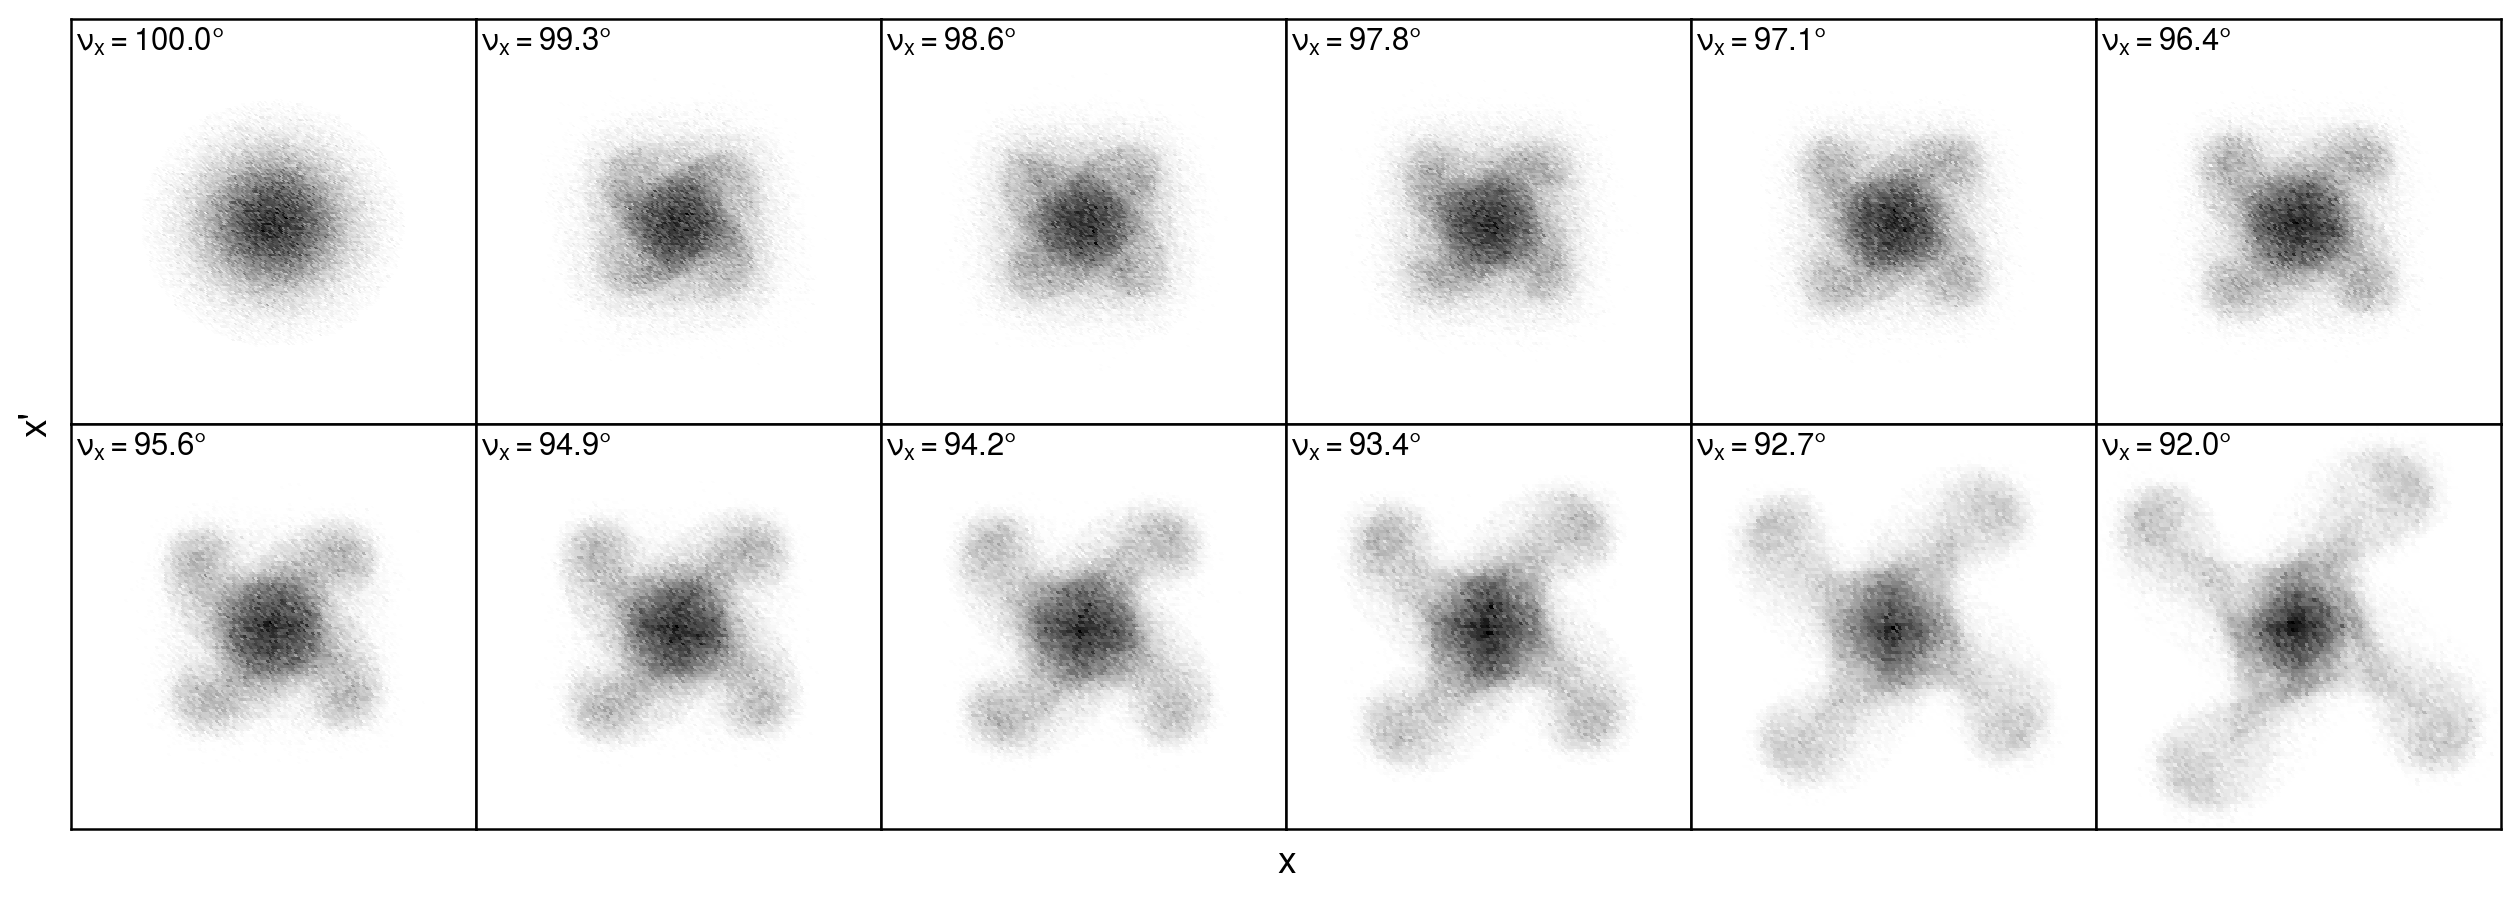
\includegraphics[width=\textwidth]{Images/chapter1/incoherent_resonance_fourth_order.png}
        \label{fig:incoherent_instability_a}
        \caption{}
    \end{subfigure}
    \begin{subfigure}{0.5\textwidth}
        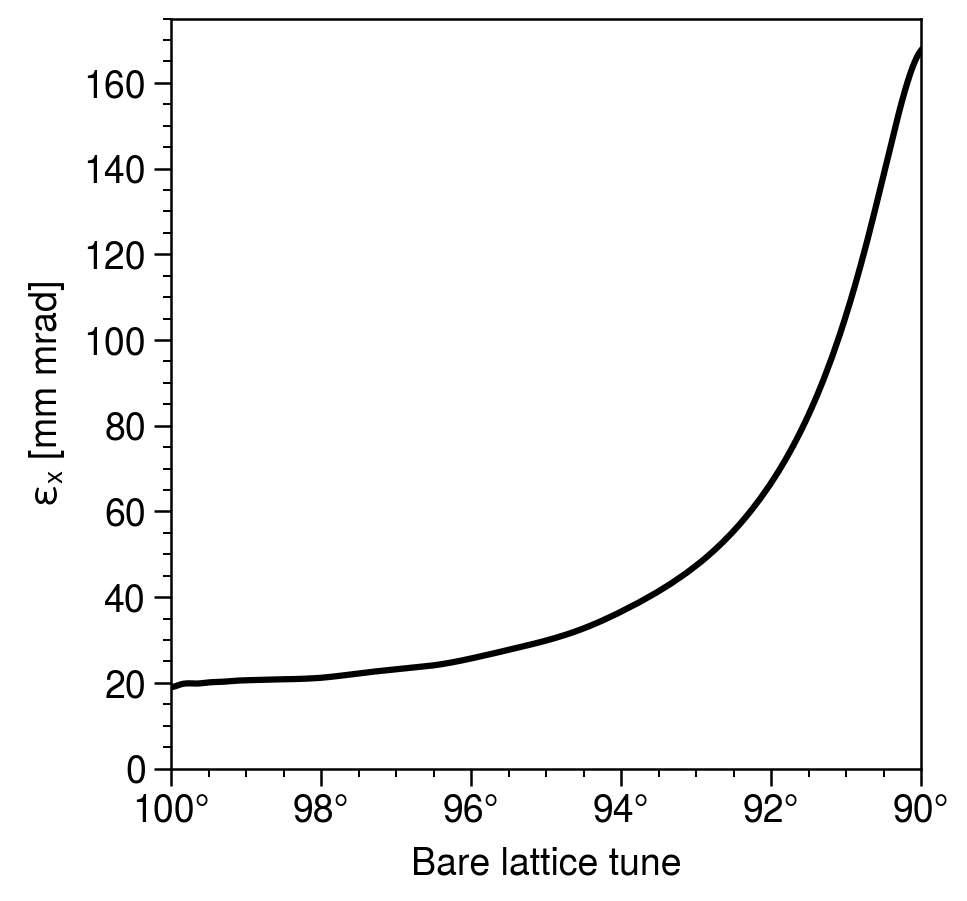
\includegraphics[width=\textwidth]{Images/chapter1/incoherent_resonance_fourth_order_emittance.png}
        \label{fig:incoherent_instability_b}
        \caption{}
    \end{subfigure}
    \caption{Simulation of a truncated Gaussian distribution in a FODO lattice. The zero-current tune is decreased from 100\degree to 90\degree over 500 cells. (a) $x$-$x'$ distribution. (b) RMS horizontal emittance. (Reproduced from \cite{Hofmann2017Book}.)}
    \label{fig:incoherent_instability}
    \vspace*{2cm}
\end{figure}
%
A fourth-order resonance is excited as the depressed tune approaches 90 degrees. The smooth emittance growth during most of the simulation shows that the core of the beam remains matched, justifying the use of ``incoherent" describe the resonance. Higher-order resonances can also occur for different combinations of beam intensity and focusing strength.





\section*{Coherent instabilities}

In \cite{Hofmann1983}, Hofmann et al. analytically studied perturbations of a round ($\varepsilon_x = \varepsilon_y$) KV distribution using the Vlasov equation in one of the simplest time-dependent cases: a FODO lattice with equal horizontal and vertical tunes. The result is shown in Fig.~\ref{fig:stopbands}, which plots the depressed tune as a function of beam intensity. Each thin line represents a different zero-current tune, and the thick lines represent regions of instability.
%
\begin{figure}[!p]
    \centering
    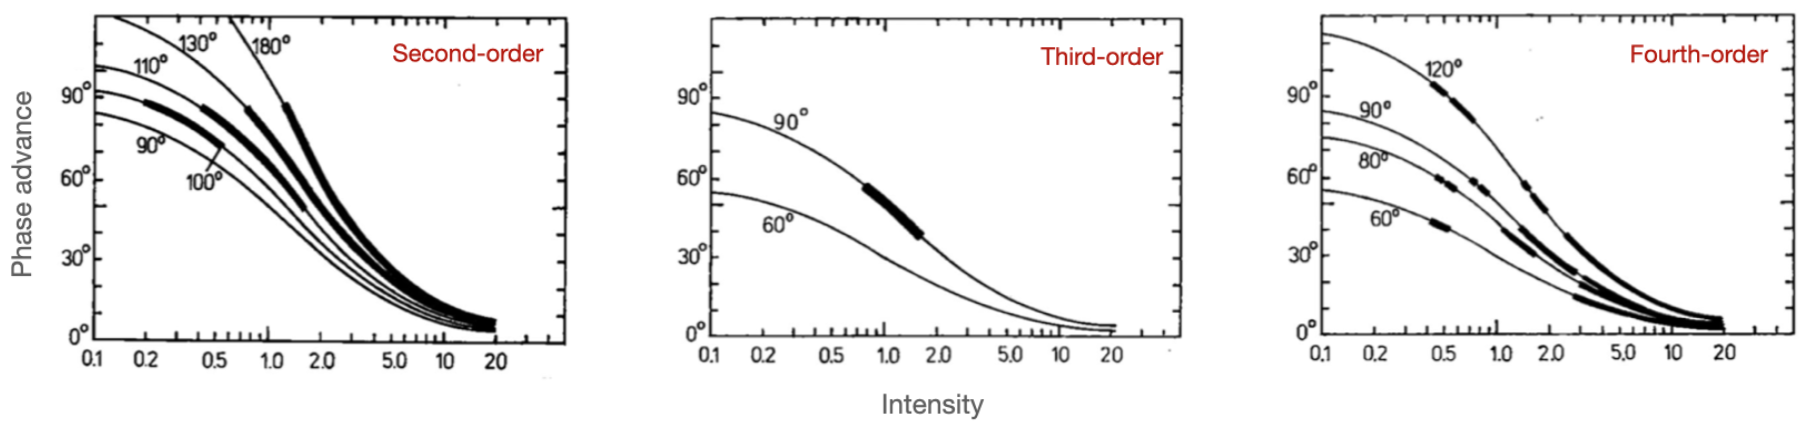
\includegraphics[width=\textwidth]{Images/chapter1/stopbands_hor.png}
    \caption{Instability stopbands obtained from perturbations of a KV distribution with equal emittances in a FODO lattice. (From \cite{Hofmann1983}).}
    \label{fig:stopbands}
\end{figure}
%

The second-order instabilities involve linear forces only, so they should appear in the KV envelope equations. We use a FODO cell with a zero-current tune of $100\degree$ corresponding to the second-to-bottom line on the left-most plot in Fig.~\ref{fig:stopbands}. The initial distribution is first matched to the lattice, then tracked for 500 cells by integrating the KV envelope equations. Fig.~\ref{fig:envelope_instability} shows the horizontal and vertical envelopes as the depressed KV tune is decreased from $90\degree$ to $71\degree$, crossing the stopband. This is known as the envelope instability. 
%
\begin{figure}[!p]
    \centering
    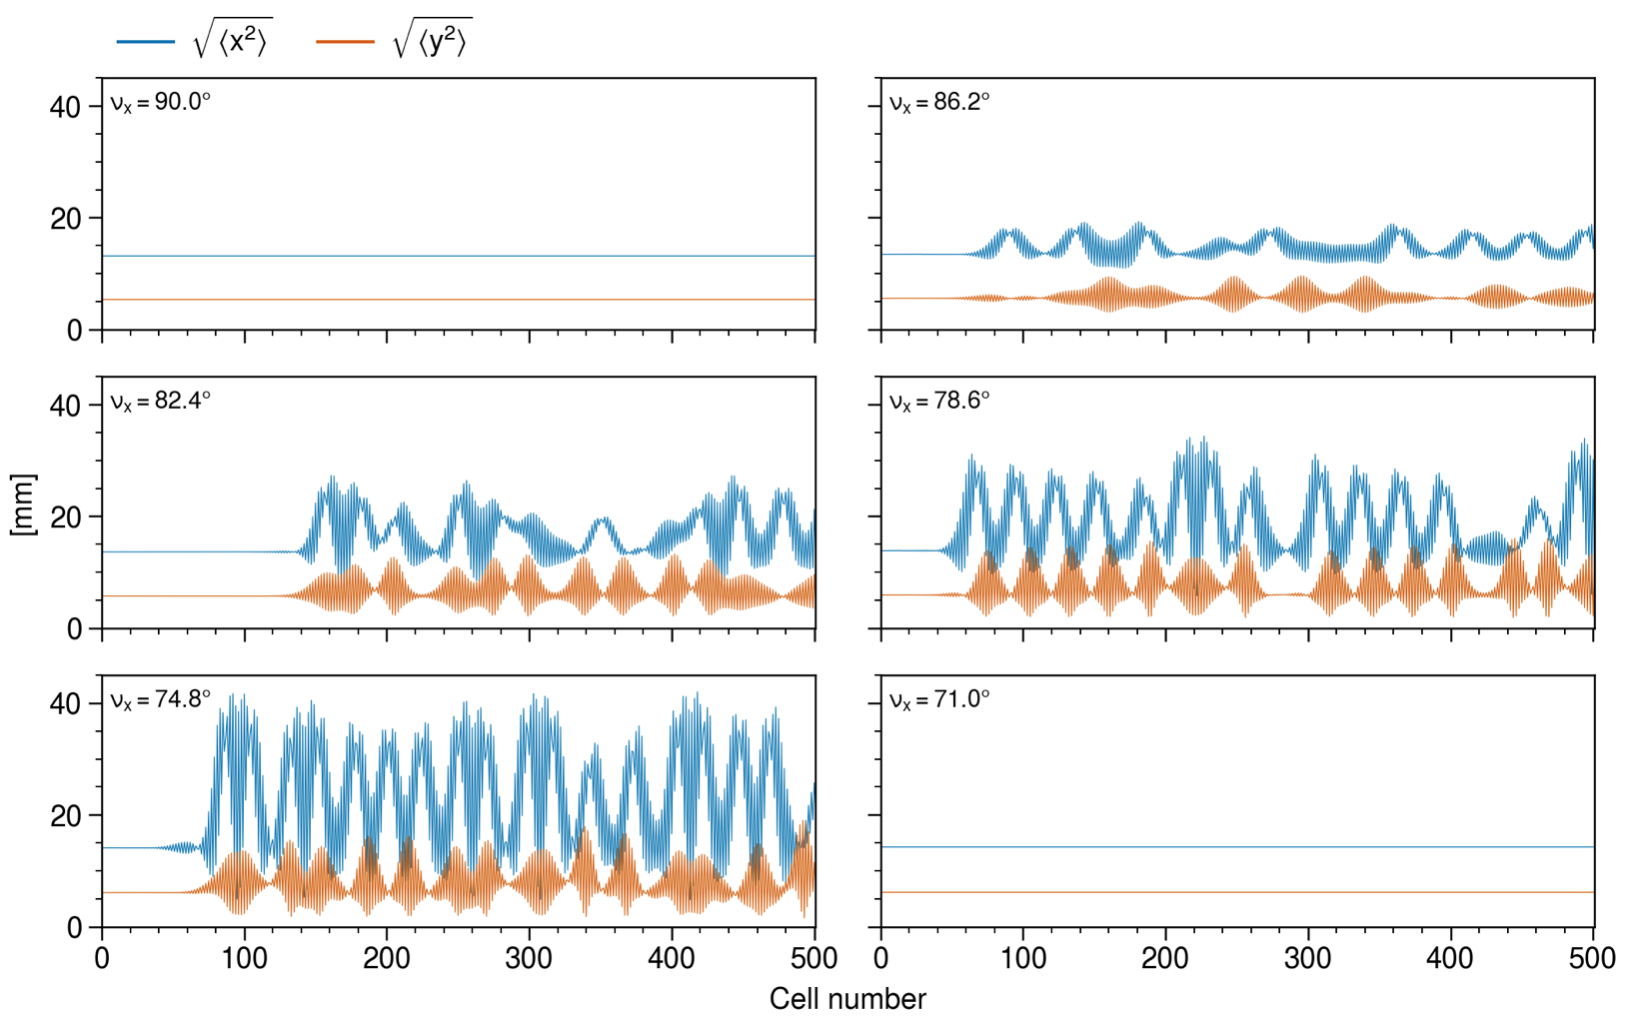
\includegraphics[width=\textwidth]{Images/chapter1/envelope_instability.png}
    \caption{Integrated KV envelope equations in a FODO lattice as the depressed KV tune $\nu_x$ is decreased. The zero-current tune is 100\degree.} \label{fig:envelope_instability}
\end{figure}
%

Observation of the higher-order stopbands requires PIC simulation. We choose a zero-current tune of 90\degree; according to Fig.~\ref{fig:stopbands}, a third-order and fourth-order instability should occur at a depressed tune of 45\degree and 30\degree, respectively. Fig.~\ref{fig:coherent_instabilities} shows the simulated evolution in PyORBIT for three different distributions: KV, Waterbag, and Gaussian. (Note that while the simulations in \cite{Hofmann2017Book} used a bunched beam, coasting beams were used in this simulation.)
%
\begin{figure}[!p]
    \begin{subfigure}[b]{0.45\textwidth}
        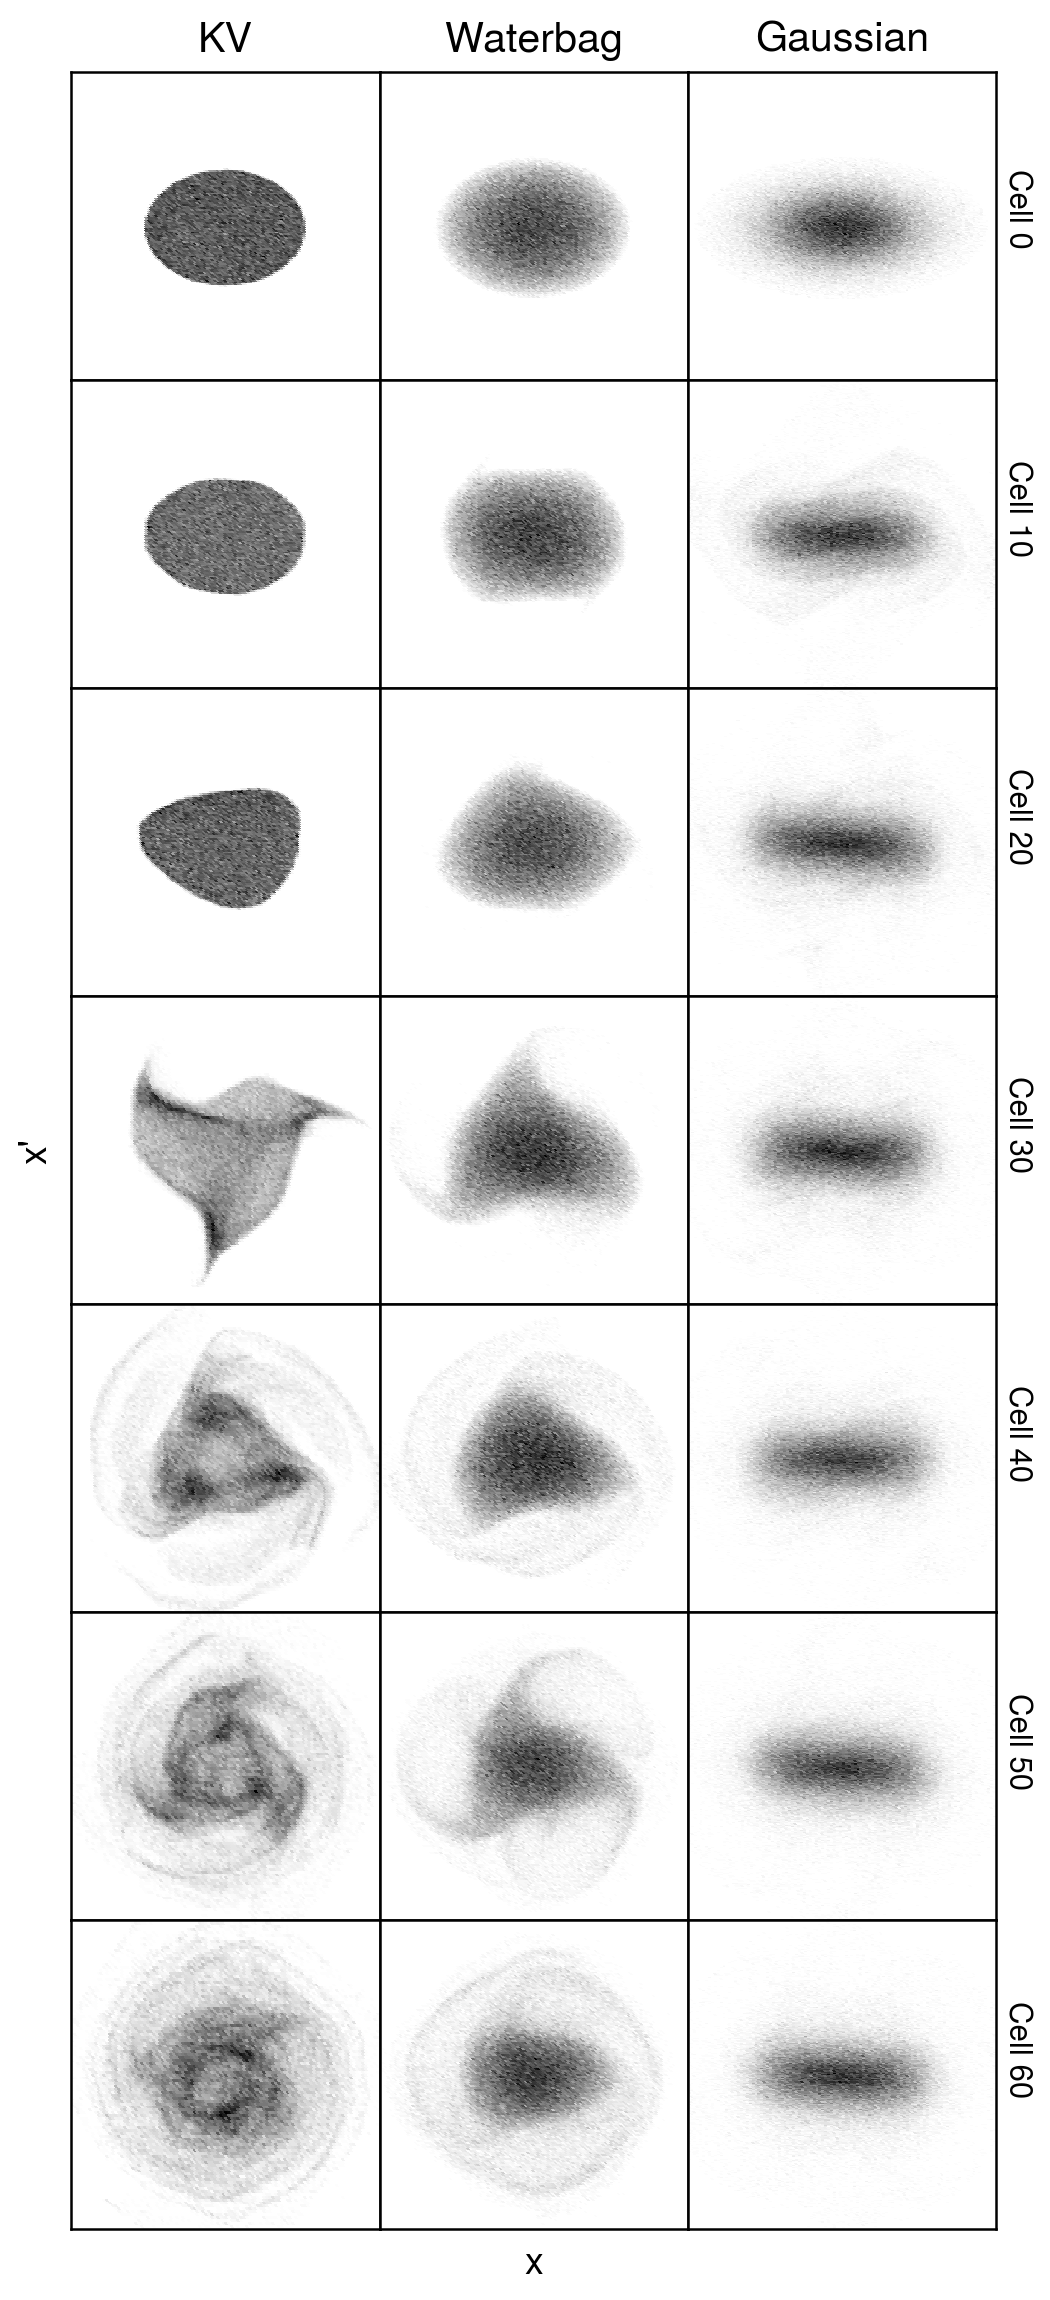
\includegraphics[width=\textwidth]{Images/chapter1/coherent_instability_fourth_order.png}
        \label{fig:coherent_instabilities_a}
    \end{subfigure}
    \hfill
    \begin{subfigure}[b]{0.45\textwidth}
        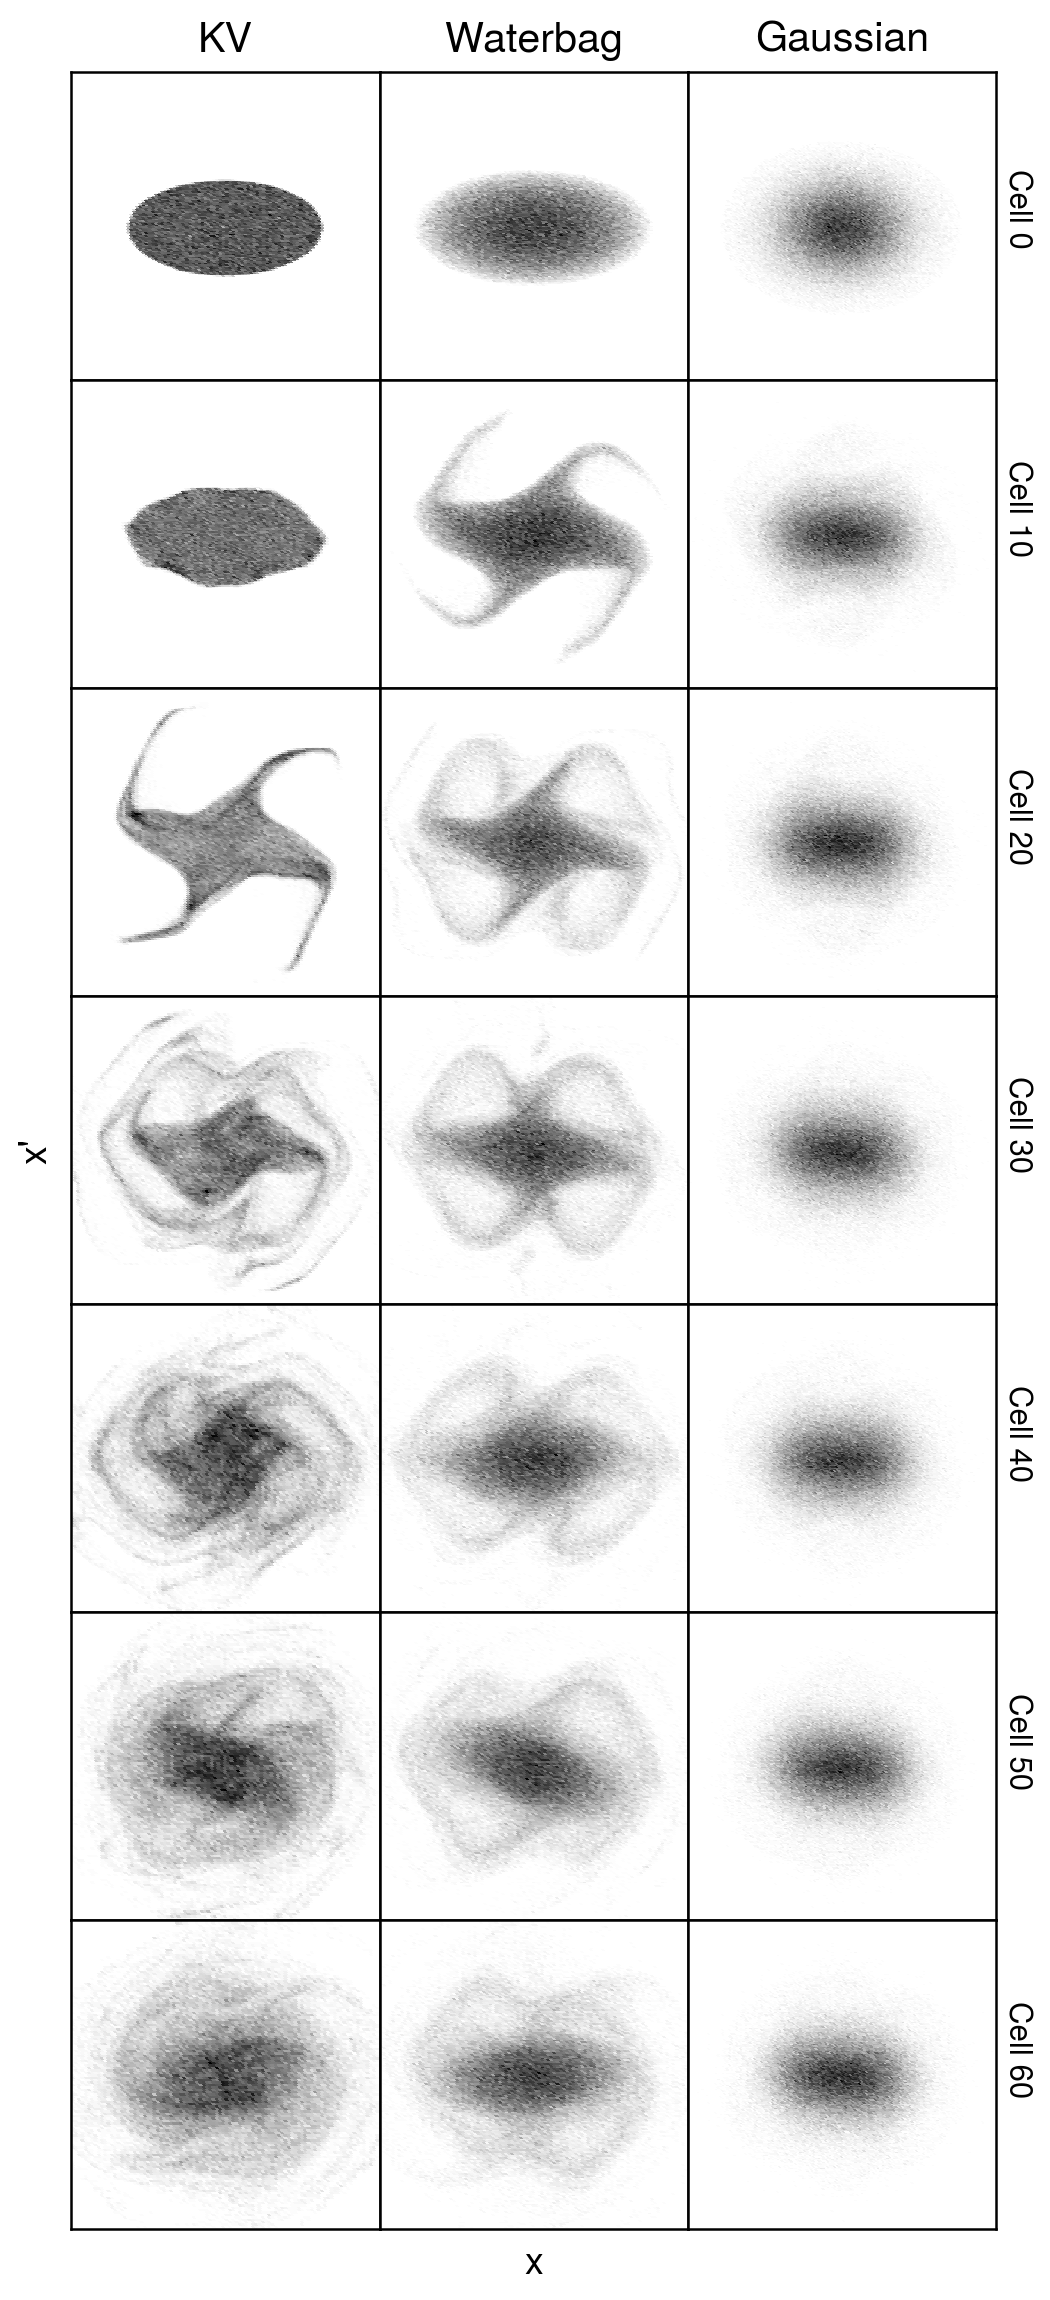
\includegraphics[width=\textwidth]{Images/chapter1/coherent_instability_third_order.png}
        \label{fig:f2}
    \end{subfigure}
    \vfill
    \begin{subfigure}[b]{\textwidth}
        \centering
        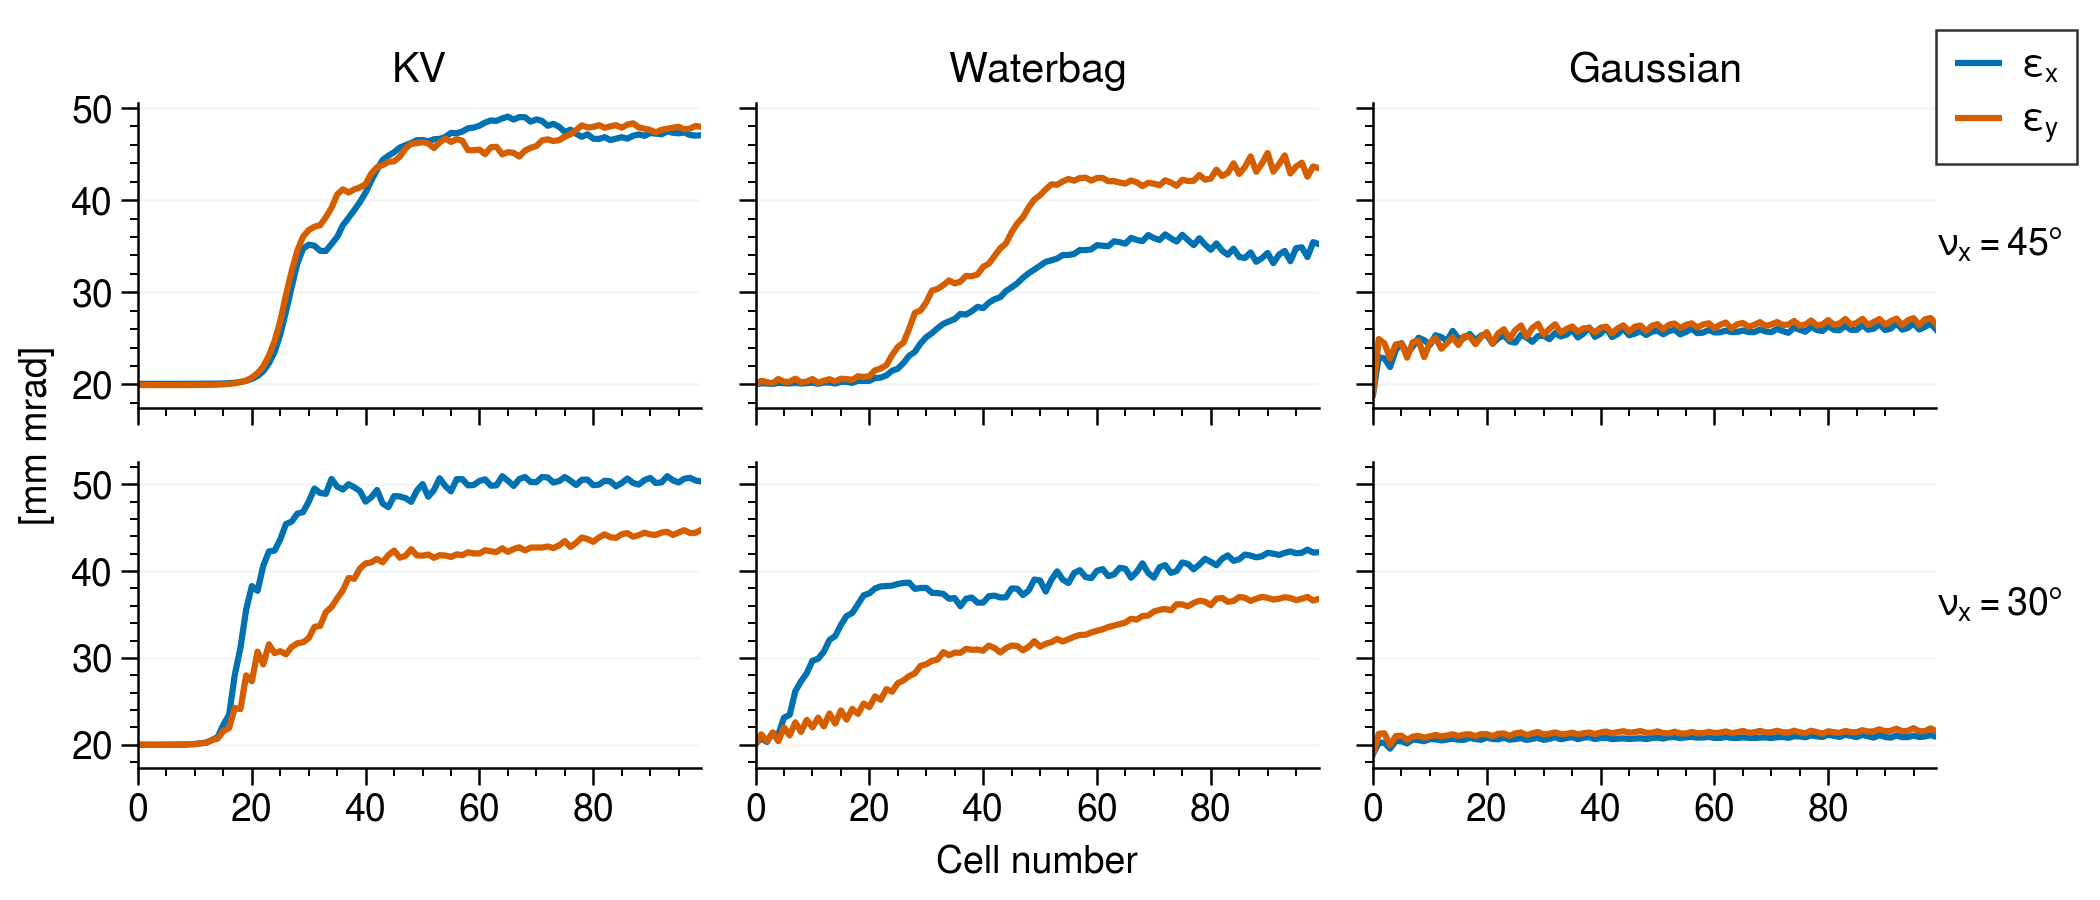
\includegraphics[width=0.8\textwidth]{Images/chapter1/coherent_instability_emittances.png}
        \label{fig:coherent_instabilities_b}
    \end{subfigure}
    \caption{Simulated Gaussian, Waterbag, and KV distributions in a FODO lattice with a zero-current tune of 90\degree and depressed KV tunes of $\nu_x$ = 45\degree (top left) and 30\degree (top right).}
    \label{fig:coherent_instabilities}
\end{figure}
%
The instabilities violently affect the KV distribution, but their effect is less pronounced in the other distributions. Thus, it is assumed that high-order coherent instabilities, while interesting, are not important in typical beams with large tune spreads.

The Danilov distribution and/or other self-consistent distributions may exhibit similar coherent instabilities as the KV distribution. Lund, Kikuchi, and Davidson noted this in 2009 \cite{Lund2009}:
\begin{quote}
    \textit{Although the low-order properties of the KV distribution are appealing physically, the full four-dimensional structure corresponds to a singular, hyperellipsoidal shell in phase space. For strong space charge, this singular structure drives unphysical, higher-order instabilities which limit practical use of the KV distribution for initializing simulations. The KV distribution is the only exact Vlasov equilibrium known that is a function of linear-field Courant-Snyder invariants. Danilov et al. \cite{Danilov2003} investigate alternative classes of exact kinetic equilibrium distributions for linear forces. These distributions are highly singular, and based on elementary plasma physics considerations, can be expected to be unstable (similar to the KV distribution) in regimes of high space-charge intensity.}
\end{quote}